% Opening block of the LangGraph seminar: what an agent is, why not an everything-agent in an enterprise,
% workflows as the middle path, and the rationale of this talk. Sits ahead of langgraph_agent_primer.
% Comment out the \input line in seminar_llm_langgraph_content.tex to switch off.

%%%%%%%%%%%%%%%%%%%%%%%%%%%%%%%%%%%%%%%%%%%%%%%%%%%%%%%%%%%%%%%%%%%%%%%%%%%%%%%%
\begin{frame}[fragile]\frametitle{}
\begin{center}
{\Large From Agents to Workflows}

\medskip
{\small (what an agent is, and why this talk is about workflows)}
\end{center}
\end{frame}

%%%%%%%%%%%%%%%%%%%%%%%%%%%%%%%%%%%%%%%%%%%%%%%%%%%
\begin{frame}[fragile]\frametitle{What Is an Agent?}
\begin{itemize}
\item An agent is something that \textbf{acts}, not only something that answers.
\item \textbf{Brain:} an LLM, ideally a reasoning model, that decides what to do next.
\item \textbf{Hands:} an array of tools: APIs, functions, database queries, actions in other systems.
\item \textbf{Loop:} keep going until the work is finished, instead of stopping after one reply.
\item Example: ``Why did pump P-104 trip last night?'' The agent reads the alarm log, pulls the vibration history, compares with the maintenance record, and drafts a finding.
\end{itemize}
\end{frame}

%%%%%%%%%%%%%%%%%%%%%%%%%%%%%%%%%%%%%%%%%%%%%%%%%%%
\begin{frame}[fragile]\frametitle{The Loop: Reason, Act, Observe, Repeat}
\begin{center}
\adjustbox{max width=\linewidth, max totalheight=0.45\textheight}{%
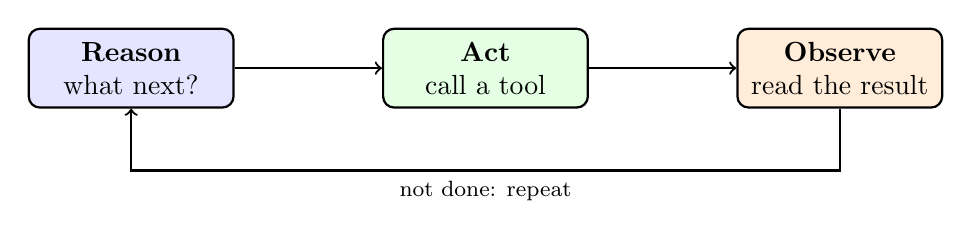
\begin{tikzpicture}[box/.style={draw, rounded corners, thick, minimum width=2.6cm, minimum height=1cm, align=center, fill=blue!10}]
\node[box] (r) at (0,0) {\textbf{Reason}\\what next?};
\node[box, fill=green!10] (a) at (4.5,0) {\textbf{Act}\\call a tool};
\node[box, fill=orange!15] (o) at (9,0) {\textbf{Observe}\\read the result};
\draw[->, thick] (r) -- (a);
\draw[->, thick] (a) -- (o);
\draw[->, thick] (o) -- ++(0,-1.3) -| node[pos=0.25, below] {\footnotesize not done: repeat} (r);
\end{tikzpicture}}
\end{center}
\begin{itemize}
\item This is the \textbf{ReAct} pattern (reasoning plus acting): the model thinks, calls a tool, reads what came back, and thinks again.
\item The loop ends when the model judges the task complete.
\end{itemize}
\end{frame}

%%%%%%%%%%%%%%%%%%%%%%%%%%%%%%%%%%%%%%%%%%%%%%%%%%%
\begin{frame}[fragile]\frametitle{One Run of the Loop: A Maintenance Report}
\begin{itemize}
\item \textbf{Task:} ``Summarise this week's unplanned stops on Line 3.''
\item \textbf{Reason:} I need the stop events first. \textbf{Act:} query the downtime log.
\item \textbf{Observe:} 14 events, 3 of them on the same press.
\item \textbf{Reason:} check that press's recent work orders. \textbf{Act:} query the maintenance system.
\item \textbf{Observe:} a lubrication task is overdue. \textbf{Reason:} enough to write. \textbf{Act:} draft the report.
\item The model chose every step. That freedom is the power, and, as the next frames show, the risk.
\end{itemize}
\end{frame}

%%%%%%%%%%%%%%%%%%%%%%%%%%%%%%%%%%%%%%%%%%%%%%%%%%%
\begin{frame}[fragile]\frametitle{Why Not Let Agents Do Anything and Everything?}
\begin{itemize}
\item A general agent that can handle any request in an enterprise needs the \textbf{largest models}, since it must reason about anything.
\item It uses \textbf{many tokens}: long prompts, many tool descriptions, many loop turns, each turn re-reading the history.
\item So the \textbf{cost} per task is high, and the \textbf{latency} is long, because every turn is a model call.
\item The path is chosen at run time, so the behaviour is \textbf{unpredictable}: the same request can take different routes.
\end{itemize}
\end{frame}

%%%%%%%%%%%%%%%%%%%%%%%%%%%%%%%%%%%%%%%%%%%%%%%%%%%
\begin{frame}[fragile]\frametitle{The Enterprise Problem: Test, Audit, Trust}
\begin{itemize}
\item \textbf{Hard to test:} there is no fixed set of paths to cover, so a test suite proves little.
\item \textbf{Hard to audit:} a regulator or a plant manager asks ``why did it do that?'' and the honest answer is a long transcript.
\item \textbf{Errors compound:} one wrong observation early in the loop can steer every later step.
\item \textbf{Broad access is risky:} an agent with many tools can also take the wrong action, such as closing the wrong work order.
\item Enterprises want automation that is \textbf{bounded, repeatable and explainable}.
\end{itemize}
\end{frame}

%%%%%%%%%%%%%%%%%%%%%%%%%%%%%%%%%%%%%%%%%%%%%%%%%%%
\begin{frame}[fragile]\frametitle{Workflows: Semi-Deterministic by Design}
\begin{itemize}
\item In most enterprise tasks the \textbf{standard procedure is already known}: triage, check, decide, record, notify.
\item Yet the steps are not trivial: reading a free-text complaint, breaking a task into parts, or judging a severity still needs \textbf{reasoning}.
\item A \textbf{workflow} keeps the skeleton fixed in code and lets the model think \emph{inside} the steps.
\item Example, ticket triage: classify the ticket, look up the asset, draft a reply, route to the right team. The order is fixed; each step uses a model.
\end{itemize}
\end{frame}

%%%%%%%%%%%%%%%%%%%%%%%%%%%%%%%%%%%%%%%%%%%%%%%%%%%
\begin{frame}[fragile]\frametitle{A Spectrum: Single Call, Workflow, Agent}
\begin{center}
\adjustbox{max width=\linewidth, max totalheight=0.4\textheight}{%
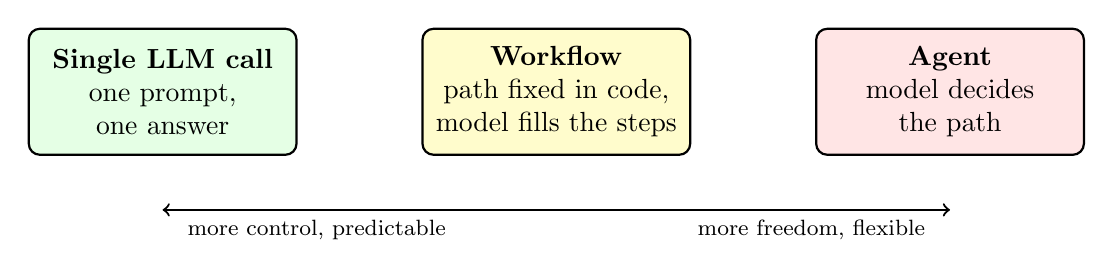
\begin{tikzpicture}[box/.style={draw, rounded corners, thick, minimum width=3.4cm, minimum height=1.6cm, align=center}]
\node[box, fill=green!10] (s) at (0,0) {\textbf{Single LLM call}\\one prompt,\\one answer};
\node[box, fill=yellow!20] (w) at (5,0) {\textbf{Workflow}\\path fixed in code,\\model fills the steps};
\node[box, fill=red!10] (g) at (10,0) {\textbf{Agent}\\model decides\\the path};
\draw[<->, thick] (0,-1.5) -- node[below] {\footnotesize more control, predictable \hspace{3cm} more freedom, flexible} (10,-1.5);
\end{tikzpicture}}
\end{center}
\begin{itemize}
\item Moving right gives flexibility; moving left gives predictability, lower cost and easier testing.
\end{itemize}
\end{frame}

%%%%%%%%%%%%%%%%%%%%%%%%%%%%%%%%%%%%%%%%%%%%%%%%%%%
\begin{frame}[fragile]\frametitle{Workflow versus Agent: The Published Distinction}
\begin{itemize}
\item Anthropic's ``Building effective agents'' draws the line this way:
\begin{itemize}
\item Workflows are ``systems where LLMs and tools are orchestrated through predefined code paths.''
\item Agents are ``systems where LLMs dynamically direct their own processes and tool usage.''
\end{itemize}
\item It advises ``finding the simplest solution possible, and only increasing complexity when needed.''
\item It notes that agentic systems ``often trade latency and cost for better task performance.''
\end{itemize}
{\tiny Source: anthropic.com/engineering/building-effective-agents (fetched October 2026).}
\end{frame}

%%%%%%%%%%%%%%%%%%%%%%%%%%%%%%%%%%%%%%%%%%%%%%%%%%%
\begin{frame}[fragile]\frametitle{A Workflow Picture: Ticket Triage}
\begin{center}
\adjustbox{max width=\linewidth, max totalheight=0.5\textheight}{%
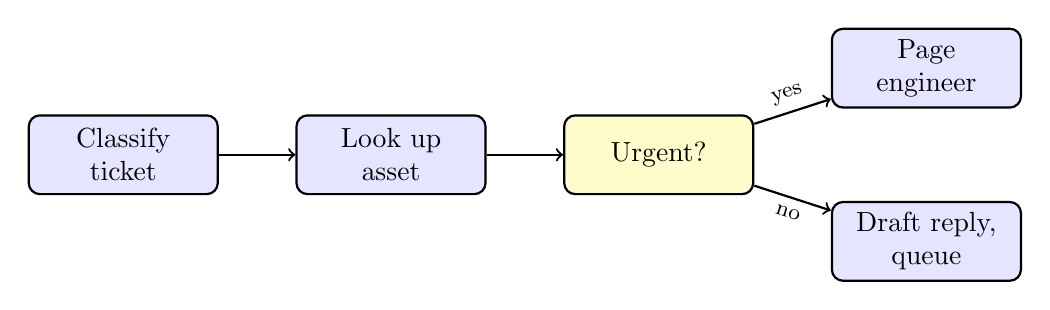
\begin{tikzpicture}[box/.style={draw, rounded corners, thick, minimum width=2.4cm, minimum height=1cm, align=center, fill=blue!10}]
\node[box] (c) at (0,0) {Classify\\ticket};
\node[box] (l) at (3.4,0) {Look up\\asset};
\node[box, fill=yellow!20] (d) at (6.8,0) {Urgent?};
\node[box] (e) at (10.2,1.1) {Page\\engineer};
\node[box] (q) at (10.2,-1.1) {Draft reply,\\queue};
\draw[->, thick] (c) -- (l);
\draw[->, thick] (l) -- (d);
\draw[->, thick] (d) -- node[above, sloped] {\footnotesize yes} (e);
\draw[->, thick] (d) -- node[below, sloped] {\footnotesize no} (q);
\end{tikzpicture}}
\end{center}
\begin{itemize}
\item The map is drawn by the developer; the model reasons inside each box.
\end{itemize}
\end{frame}

%%%%%%%%%%%%%%%%%%%%%%%%%%%%%%%%%%%%%%%%%%%%%%%%%%%
\begin{frame}[fragile]\frametitle{Why This Talk: LangGraph Builds Workflows}
\begin{itemize}
\item LangGraph expresses a workflow as a \textbf{graph}: \textbf{nodes} (steps), \textbf{edges} (what follows what) and a \textbf{shared state} passed along.
\item \textbf{Explicit control flow:} branching and loops are drawn, not left to the model's mood.
\item \textbf{Checkpoints} save the state after each step, so a run can be resumed, replayed and inspected.
\item \textbf{Human in the loop:} pause at a node, let a person approve or edit, then continue.
\item A node can be plain code, one LLM call, or a whole small agent, so you choose the autonomy per step.
\end{itemize}
\end{frame}

%%%%%%%%%%%%%%%%%%%%%%%%%%%%%%%%%%%%%%%%%%%%%%%%%%%
\begin{frame}[fragile]\frametitle{Where Enterprise Value Is Likely to Grow}
\begin{itemize}
\item \textbf{Opinion, not a measured result:} workflows may deliver more enterprise value than generic foundation-model agents.
\item A narrow, well-defined task (classify a ticket, extract fields from a report) does not need the biggest model.
\item A \textbf{smaller, task-specific model} can be \textbf{fine-tuned} on the company's own examples.
\item It can run \textbf{cheaper} and \textbf{faster}, stay \textbf{private} inside the firewall, and even run \textbf{locally}.
\item Fixed structure also gives what the previous frames asked for: testable steps and an audit trail.
\end{itemize}
\end{frame}

%%%%%%%%%%%%%%%%%%%%%%%%%%%%%%%%%%%%%%%%%%%%%%%%%%%
\begin{frame}[fragile]\frametitle{Frugal AI: The Least Compute That Does the Job}
\begin{itemize}
\item \textbf{Frugal AI} is the habit of choosing the smallest model and the simplest structure that meets the need.
\item Start with a single call; add a workflow when steps are known; add agent freedom only where it clearly pays.
\item Use code for what code does well, and the model only for the part that needs language or judgment.
\item The rest of this talk shows how to build such workflows, step by step, with LangGraph.
\end{itemize}
\end{frame}
